The objective of our case study is a comparative analysis of the two environments and to find out if there exists software performance regression between a dedicated server and the virtual environment. To analyze this, we divided our project into three research questions. Following the set up of the subject systems and data preprocessing, we used requests per minute as our independent variable and performance metrics as our dependent variables to answer our research questions. %Firstly, we observe if our models are transferable across the three chosen environments. Secondly, if the models can accurately predict counter values cross-servers. Lastly, if defect injection will generate similar performance metrics values compared   

\subsection{\textbf{Do performance metrics from physical and virtual environments belong to the same population?}}

\textbf{Motivation}: Performance assurance activities are not only bounded by the idea that performance regression can only be identified relative to different versions of the software. A software system might also regress once it is transferred from one environment to another. According to the norm, practitioners often rely on performance metrics generated by the virtual environment prior to releasing it on a disparate environment. We address this question by comparing the metric values between the physical and virtual server. 

\textbf{Approach}: As mentioned earlier in Section 3, after setting up the subject systems, we used the number of requests as our workload for the systems. A script was written to randomly alter the workload after every minute for CloudStore and every two minutes for DS2. The script was based on an underlying assumption that every unit of change in the performance metrics there will be a consequent unit of change in the workload which eventually introduced variety in our dataset. \cite{linearregression}. Subsequently, the requests per minute were mapped against the performance metrics recorded via \textit{perfmon}.

The numerical values for requests per minute were extracted out of the web server's access logs. These requests were recorded per second and reached up to thousands in a minute, depending on the workload. We then, with the aid of a script, grouped and extracted the requests per minute for as long as the test systems were exercised. The metrics, on the contrary, were recorded every 10 seconds. A set of six records was averaged out as a minute according to the timestamps. This was called a single \textit{run}. The metrics generated for the web and database server were concatenated. Ultimately, we had a dataset consisting of 500 runs where every record represented a \textit{run}; the metrics and requests generated for a given minute. This process was carried out for both of our environments. The two datasets, to analyze any discrepancies, were then analyzed using R's q-q plots and \textit{cor} function.

\begin{figure}[thb]
	\centering
	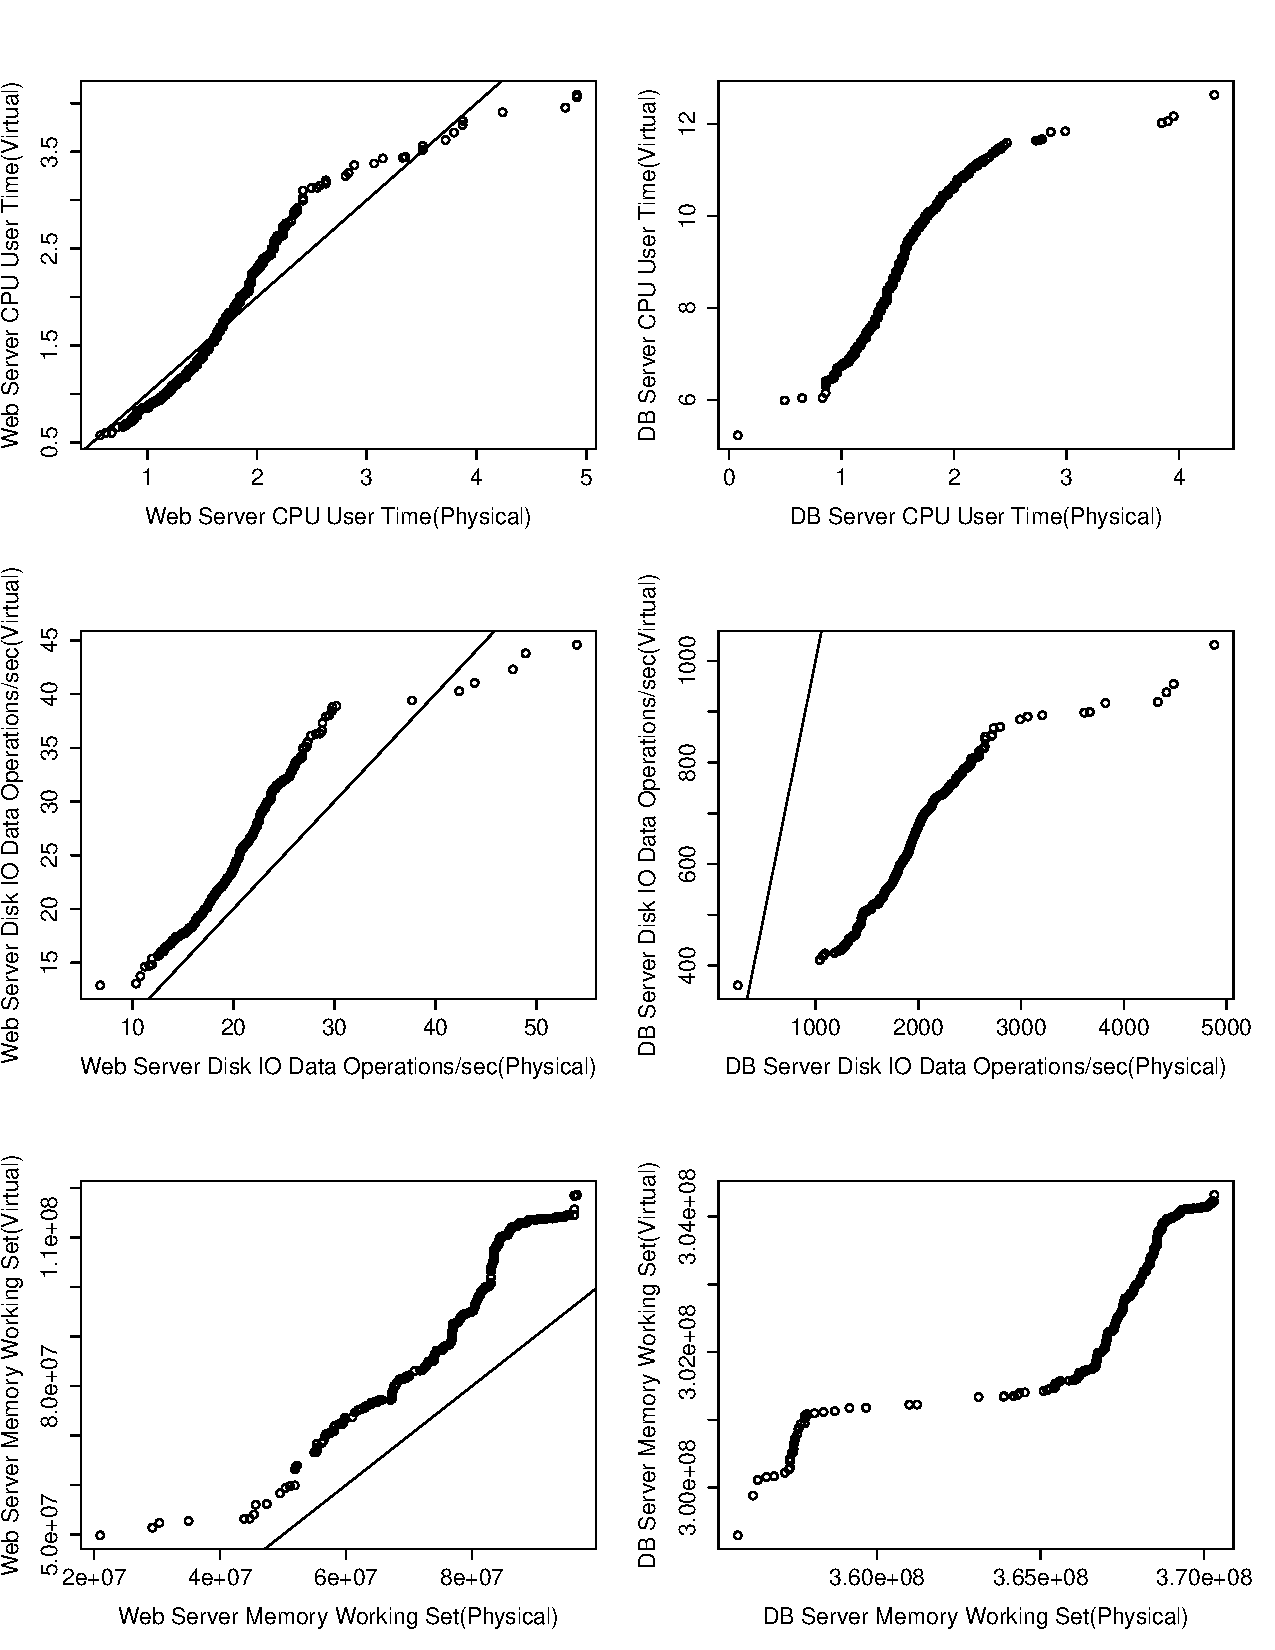
\includegraphics[width=0.9\columnwidth]{figures/ds2_qq.pdf}
	\caption{Q-Q plots: DS2}
%	\captionsetup{justification=centering}
	\label{fig:Results Table}
\end{figure}



\begin{figure}[thb]
	\centering
	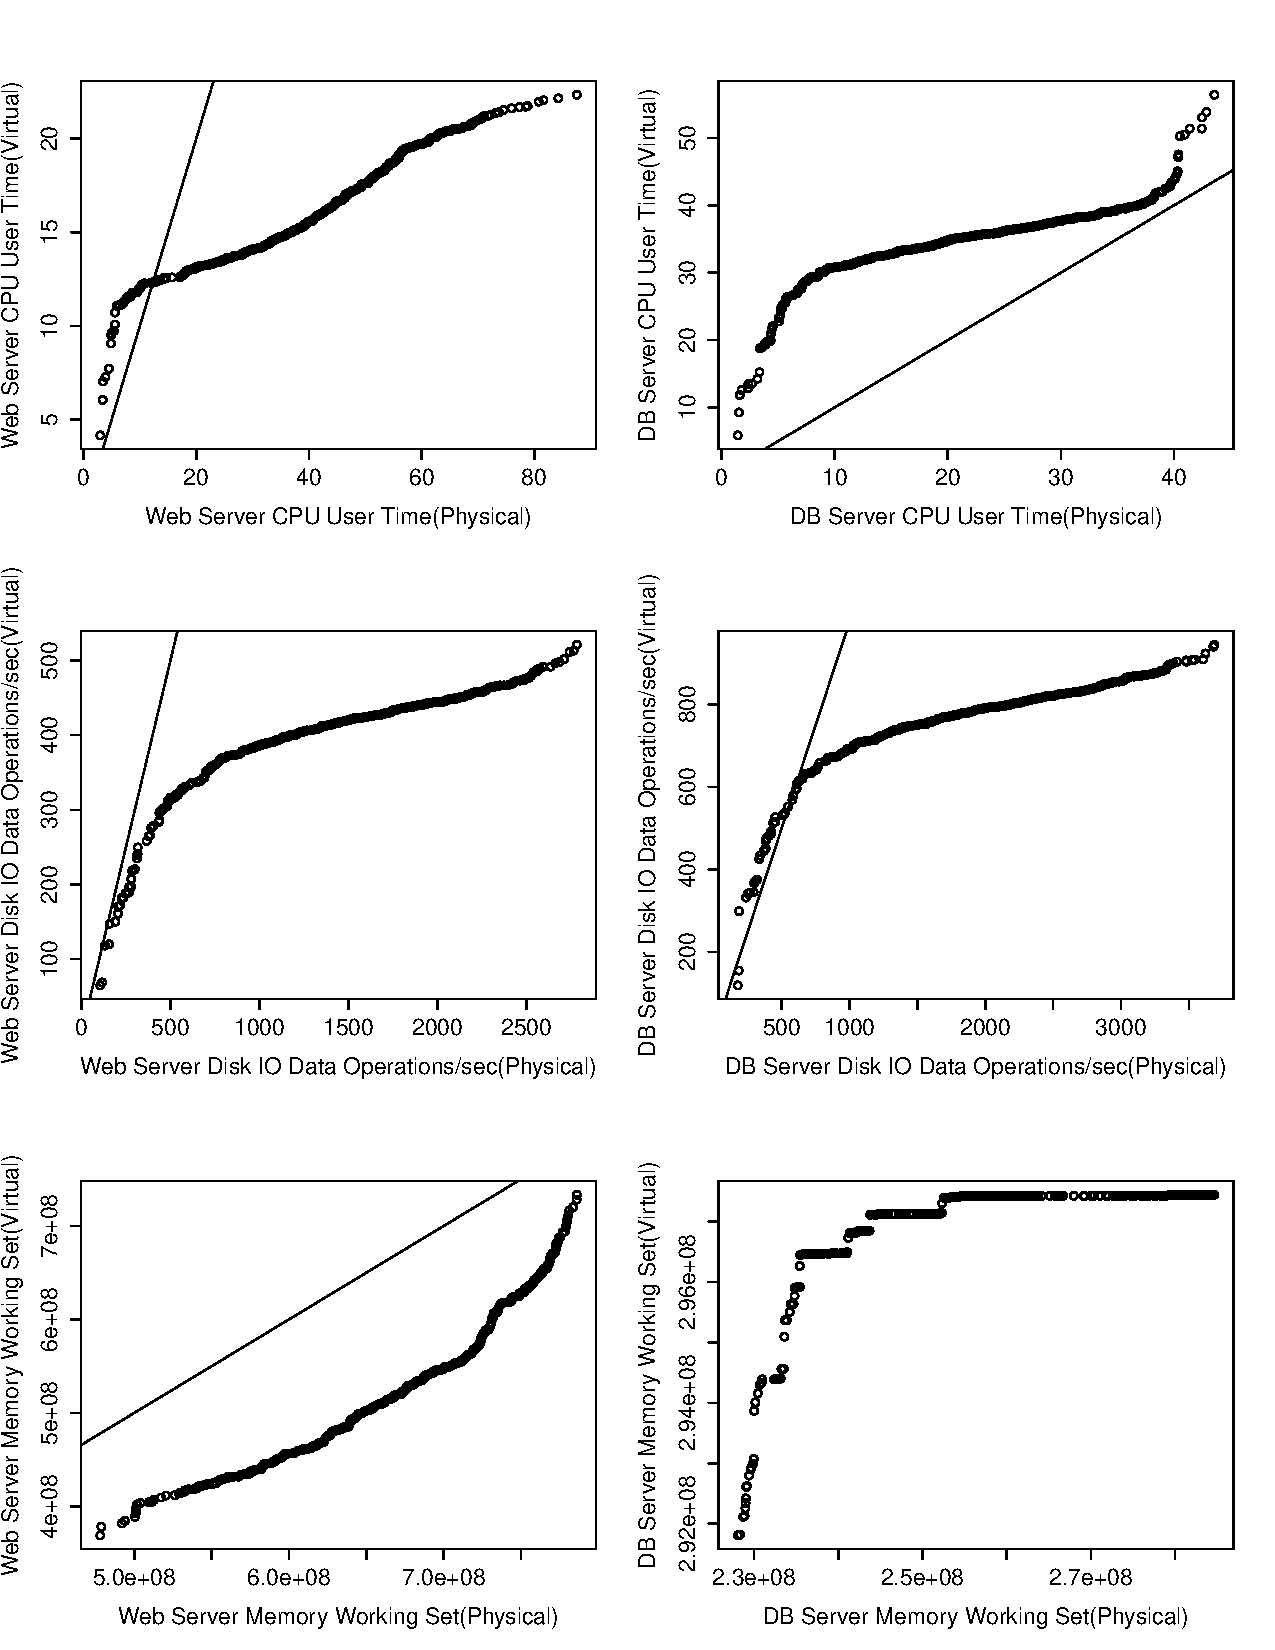
\includegraphics[width=0.9\columnwidth]{figures/cloudstore_qq.pdf}
	\caption{Q-Q plots: CloudStore}
%	\captionsetup{justification=centering}
	\label{fig:Results Table}
\end{figure}



\begin{table}[t]
	\centering
			\caption{DS2: Correlation Values}
			\label{resultRQ3}
	\begin{tabular}{c|cc}
				\textbf{Performance Metrics}   & \textbf{Cor} & \textbf{p-value}\\  
			 
				\textbf{Web Servers' User Times} &  0.08 & 0.07\\
				\textbf{DB Servers' User Times} & -0.05 & 0.30\\
				\textbf{Web Servers' IO Data Ops/Sec}   & 0.25 & 0.000 \\
				\textbf{DB Servers' IO Data Ops/Sec} & -0.14 & 0.00\\
				\textbf{Web Servers' Memory Working Set} & 0.22 & 0.00\\
				\textbf{DB Servers' Memory Working Set} & 0.46 & 0.00\\
		\end{tabular}
\end{table}
	
\begin{table}[t]
		\caption{CloudStore: Correlation Values}
		\label{resultRQ3}
		\begin{tabular}{c|cc}
			\toprule
			\textbf{Performance Metrics}   & \textbf{Cor}& \textbf{p-value}\\
			\midrule 
			\midrule 
			\textbf{Web Servers' User Times} & \ 0.01& 0.87\\
			\textbf{DB Servers' User Times} & \ 0.20 & 0.00\\
			\midrule 
			\textbf{Web Servers' IO Data Ops/Sec}   & \ 0.17& 0.00 \\
			\textbf{DB Servers' IO Data Ops/Sec} & \ 0.18& 0.00\\
			\midrule 
			\textbf{Web Servers' Memory Working Set} &\ 0.69& 0.00\\
			\textbf{DB Servers' Memory Working Set} & -0.13 & 0.00\\
			\bottomrule             
		\end{tabular}
\end{table}

%\begin{figure}[t!]
%	\centering
%	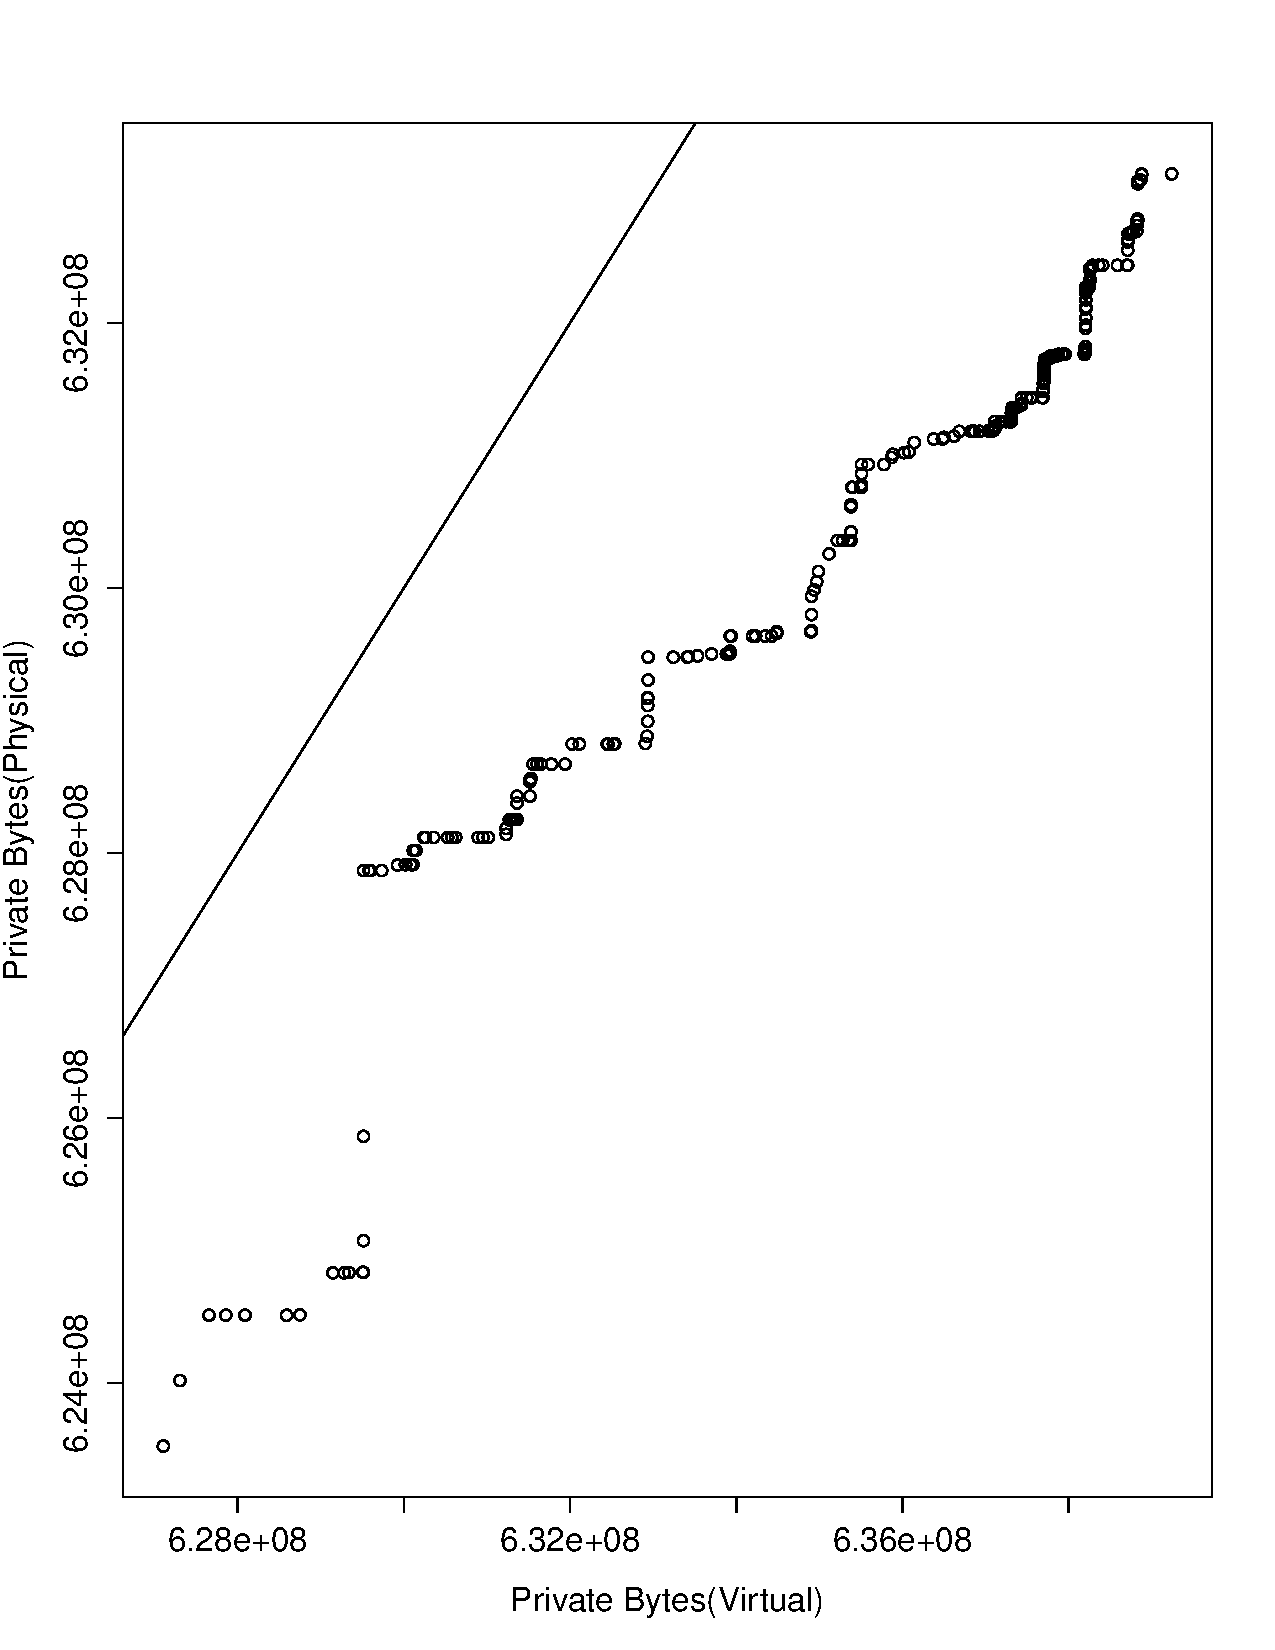
\includegraphics[width=0.7\textwidth]{private_bytes.pdf}
%	\caption{QQ-plot of Private Bytes of Physical vs. Virtual Environment}
%	\captionsetup{justification=centering}
%	\label{fig:Results Table}
%\end{figure}

%\textbf{Approach}: 
%Following our data preprocessing, we decided to use Q-Q plot to identify if there exists a similarity between the distribution of our counters for the dedicated and the virtual server. We divided our metrics into three sub-categories namely \textit{processor, IO and memory}.

\textbf{Results}: Figure 2 and 3 show the results from our q-q plots. For the sake of brevity, we chose one q-q plot to be displayed from each subset of metrics i.e. CPU, IO and memory. If the distributions of our performance metrics were similar, we should see the plots closer to the line y=x. For the sake of reference, we named this line 'Z'. \cite{Cross_Validation}. We plotted the line Z on the same axes. 

As seen in Figure 2 for the subject system DS2, the CPU user times for the web servers are closer to the line Z however the plots database servers' CPU user times are highly deviated from the same line as it not visible in the same plot. The disk IO operations/sec for the web servers gradually deviate form the line Z whereas the database server is, again, highly deviated. The same can be concluded about the memory working sets for both of our environments.
Figure 3 shows the q-q plots for CloudStore. The web servers CPU user times are not congruent with the line Z. The database server CPU user times towards the tail of the plot are closer to the line Z however they still do not follow the line Z. The disk IO operations for both servers tends to follow the line Z initally but gradually moves away. Further on, the memory working set for both of our servers, as seen, are distant to the line Z.

Our Mann-Whitney \textit{U} Tests also concluded that for each of the performance metrics selected they do not belong to the same distributions with a p-value $<$ 0.05, except the web server's user times for DS2.

Table 1 and 2 shows the Spearman correlation values between the selected performance metrics. If the correlation value is closer to 1 the metrics have a strong correlation and if the value is closer to 0 the metrics have a weak correlation. A negative correlation means that if one of the metrics is increasing in value, the other is decreasing. For both of our subject systems we observe that the correlation values are mostly positive and are closer to 0 representing weak correlations. This conclusion, however, is not applicable to the user times from both environments as the p-value $>$ 0.05.

\subsection{\textbf{Is the correlation value between load and performance metrics same cross-environments?}}

\textbf{Motivation}: Building on the conclusion from the previous research question, we next address the change in metric correlation values amongst themselves and versus the load. Our goal was to explore whether the change in correlation cross-environments is identical for both of our subject systems. This way we will be able to conclude whether a certain type of discrepancy is always present between the two environments or is it the unstable nature of the performance of subject systems in different environments. 
%Before the software is deployed in a physical environment, the performance analyst relies on the heuristics generated from the virtual environment \cite{foo2010mining}. One of the approaches to detect performance regression is to compare every metric with the previously passed performance test \cite{Shang:2015:ADP:2668930.2688052}. As discussed in our previous research question, most of the performance metrics between two environments do not belong to the similar distribution. 

%As discussed in RQ1, we discovered that our comparison of performance metrics between our physical and virtual environments produced dissimilar results. Our next step was to explore what metrics changed the most 


%As performance testing spans our from handful of hours to several days , the reliability on such exercise is remarkably critical. A recent bug fix or a modification may require a reiteration of performance tests \cite{foo2010mining}. On the contrary, This led us to our next question, that whether the performance assurance activities run on virtual environments can be duplicated.

\textbf{Approach}: We looked for the top 5 metrics which are highly correlated with the load in each of our environments. We used R's \textit{cor} function to determine the Spearman value of the aforementioned associations. 
Next, we used heat maps to highlight the set of metrics which show a significant change in correlation values amongst themselves.
The correlation values between the metrics of physical server were stored in matrix A. The correlation values between the metrics of the virtual server were store in matrix B. Matrix Z was the absolute difference between these two matrices. For example the Spearman correlation value for CloudStore's physical server between web server's User Time and database server's IO write/Bytes sec is 0.94. The correlation value for the same pair of metrics in the virtual environment is 0.26. Then the Matrix Z will record a value which is the absolute difference of the aforementioned Spearman values i.e. 0.68. If the metric value has changed significantly, according to the legend, this will be denoted as a 'hot zone' in the heatmap denoted by a lighter gradient of color.

\textbf{Results}: Figure 4 and 5 are the heatmaps for the change in correlation values amongst the metrics of two environments. For DS2, figure 4, the hot spots are mostly prevalent between the IO operations, for both the web and database server, cross-environments. This means the correlations amongst IO operations in the physical environment are not the same as the correlation between IO operations in the virtual environment. While CloudStore's heatmap, figure 5, shows that the change in correlation values is not as similar to DS2. Most of the hot spots are scattered across the heatmaps, contrary to DS2 where we can see clusters around most of the IO operations. 

We also observed a similar change in correlation values between the processor times and other metrics. This trend may not be as strong as CloudStore's heatmap for DS2, however these changes in values can be found in both of our subject system.

Table 3-6 are the top five highly correlated metrics with the load. In DS2, most of the IO operations from the web driver are highly correlated with the load in the physical environment. However, the database server is highly correlated than any of the metrics from the web driver in the virtual environment.
Table 5 and 6 shows a much similar behavior of CloudStore in both the environments.

We primarily learned that the DS2 IO operations' behavior in one environment are not similar to that of the physical environment. We also learned that the change in nature of correlation cross-environments is non-uniform.
%Figure 4 and 5 are the heatmaps for the change in correlations' values between the metrics of two environments. For DS2, figure 4, 4he hot spots are mostly prevalent between the IO operations cross-environment while CloudStore's heatmap, figure 5, shows that the change in correlation values is not as similar to DS2. Most of the hot spots are scattered across the heatmaps, contrary to DS2 where we can see clusters around most of the IO operations.



\begin{figure}[tbh]
	\centering	
	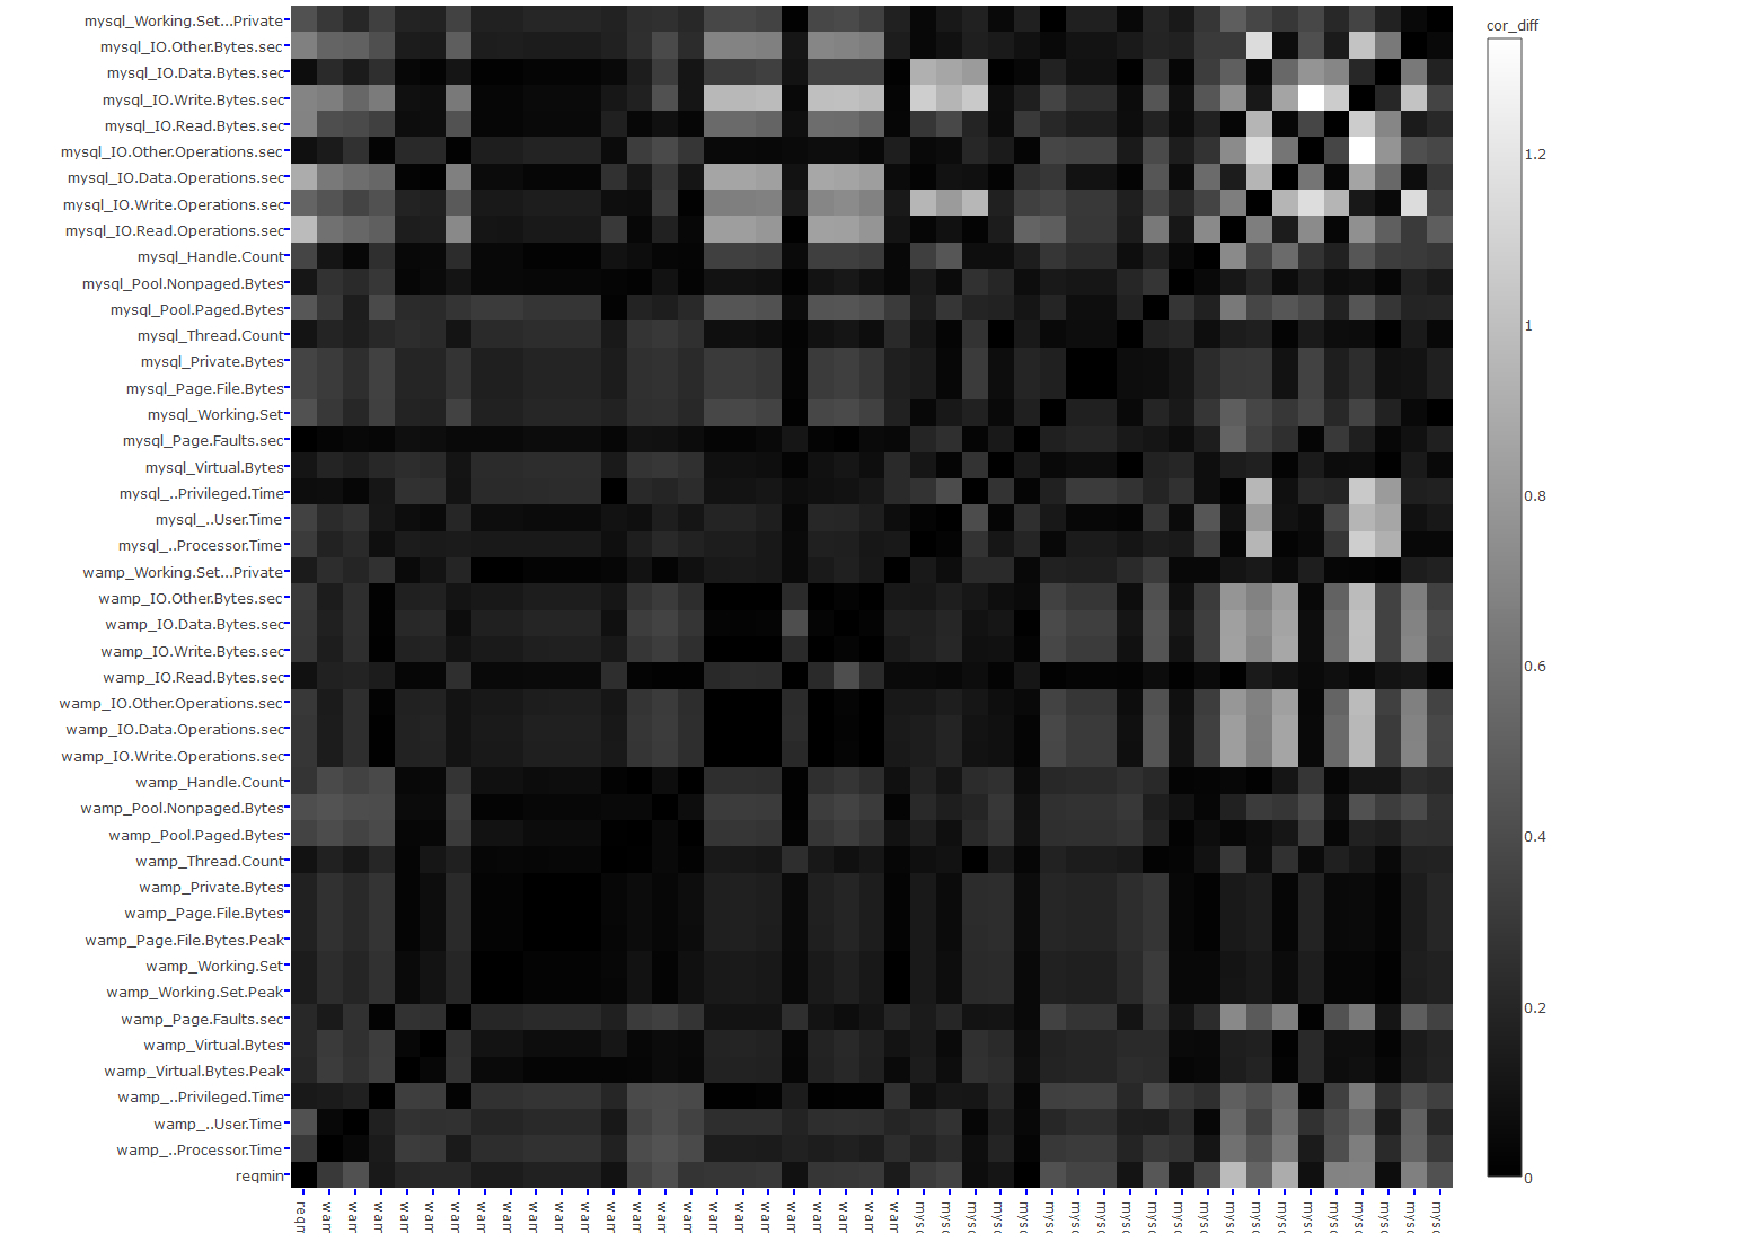
\includegraphics[width=0.5\textwidth]{figures/ds2_heatmap.pdf}
	\caption{Heatmap: DS2}
%	\captionsetup{justification=centering}
	\label{fig:Results Table}
\end{figure}

\begin{figure}[tbh]
	\centering
	{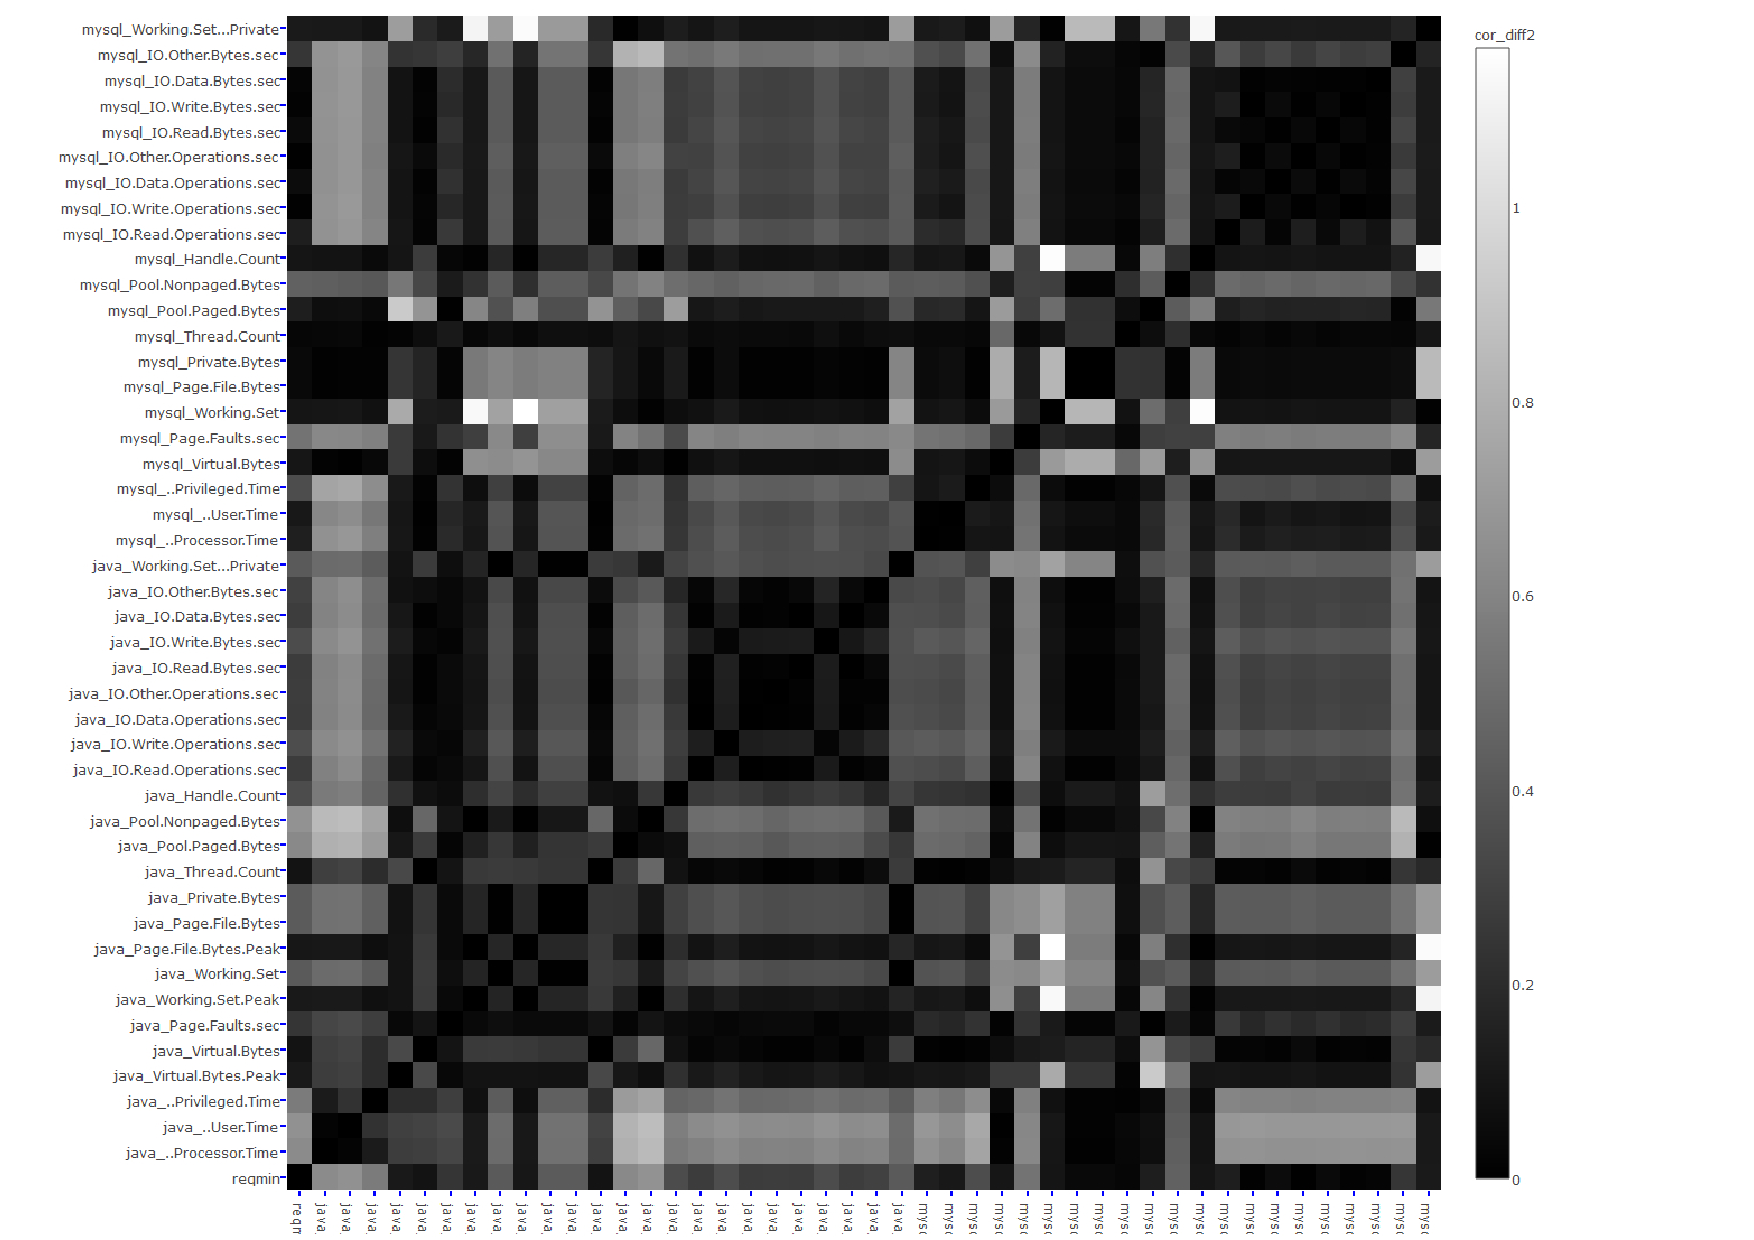
\includegraphics[width=0.5\textwidth]{figures/cloudscale_heatmap.pdf}}
	\caption{Heatmap: CloudStore}
	%\captionsetup{justification=centering}
	\label{fig:Results Table}
\end{figure}


\begin{table}[tbh]
		\centering
		\caption{DS2: Top 5 highly correlated metrics with load (Physical Server)}
		\label{resultRQ3}
		\begin{tabular}{c}
			\toprule
			1. Web Server IO Other Operations/sec \\
			2. Web Server IO Other Bytes/sec \\
			3. Web Server IO Write Operations/sec \\
			4. Web Server IO Data Operations/sec \\
			5. Web Server IO Data Bytes/sec \\
			
			\bottomrule             
		\end{tabular}
\end{table}

\begin{table}[tbh]
	\centering
		\caption{DS2: Top 5 highly correlated metrics with load (Virtual Server)}
		\label{resultRQ3}
		\begin{tabular}{c}
			\toprule
			1. Database Server Handle Count \\
			2. Database Server Working Set-Peak \\
			3. Database Server Pool Paged Bytes \\
			4. Database Server IO Other Operations/sec \\
			5. Database Server Page File Bytes Peak \\
			\bottomrule             
		\end{tabular}
\end{table}

\begin{table}[tbh]
	\centering
		\caption{CloudStore: Top 5 highly correlated metrics with load (Physical Server)}
		\label{resultRQ3}
		\begin{tabular}{c}
			\toprule
			1. Database Server IO Other Bytes/sec  \\
			2. Database Server IO Read Operations/sec   \\
			3. Database Server IO Read Bytes/sec \\
			4. Database Server IO Data Operations/sec    \\
			5. Database Server IO Write Operations/sec \\
			\bottomrule             
		\end{tabular}
\end{table}


\begin{table}[tbh]
	\centering
		\caption{CloudStore: Top 5 highly correlated metrics with load (Virtual Server)}
		\label{resultRQ3}
		\begin{tabular}{c}
			\toprule
			1. Database Server IO Other Operations/sec  \\
			2. Database Server IO Write Operations/sec   \\
			3. Database Server IO Write Bytes/sec \\
			4. Database Server IO Data Bytes/sec    \\
			5. Database Server IO Read Bytes/sec \\
			\bottomrule             
		\end{tabular}
\end{table}


\subsection{\textbf{Do performance metrics from different environments impact performance modeling?}}

\textbf{Motivation}: As discussed in earlier work \cite{Shang:2015:ADP:2668930.2688052} \cite{Nguyen:2012:ADP:2188286.2188344}, performance tests require a large dedication of resources as it is carried out just before the system is on the brink of deployment. This gives insufficient time to the performance engineers, leaving them with minimal resources. As a result they leverage on the performance assurance activities carried out in the virtual environment. The motivation behind this research question is to investigate whether the performance models generated from one environment can be applied and held representatives of the other. In essence, this will help the practitioners conclude the reliability of the performance activities carried out in the virtual environment. 
% In practice, this may or may not be appropriate to assume. This also spawns the concept of including the entire set of performance metrics for analysis, which is slipshod and ineffectual. 

\textbf{Approach}: We first validated our models with an environment using 10-fold cross validation. \textit{K}-fold cross validation divides the data into \textit{k} parts which are known as folds. The model is trained on \textit{k}-1 folds and tested on the \textit{k}$^{th}$ fold. This process is iteratively repeated \textit{k} times \cite{10foldcross} \cite{kohavi1995study}.


We partitioned our results into two segments; the explanatory and the predictive part for our models, trailed by applying our model to predict load cross-environments. The explanatory part calculates the percentage of deviance explained by our models i.e. the fit of the model while the predictive part explains the error percentage between the actual and predicted load values. Both of these parts were addressed by building generalized linear models that only incorporated the metrics which were selected via R \textit{stepwise stepwise} or commonly knows as \textit{stepwise} function, from the complete set of metrics from the dataset.

\textit{Explanatory Power}

After removing any outliers for both of our subject systems, we built our GLM, initially, using all the physical server's metrics. We trained and tested our model on the same server i.e. physical. We then reduced our model, iteratively, using only the metrics that our contributing the most to the model. This was achieved using R's \textit{stepwise} function. The \textit{stepwise} function adds the independent variables one by one to the model to exclude any metrics that not contributing to the model \cite{RInAction}. Once the metrics were automatically selected out on the physical server, we used R's \textit{ANOVA}, or \textit{analysis of deviance} to rank the metrics according to their deviance value. Higher the deviance value for a given performance metric in the model, higher the contribution of the performance metric to the model. This approach was similarly applied to the set of metrics from the virtual server to build a generalized linear model. R's \textit{deviancepercentage} was used to determine the explanatory part or fit of our model. It is used to calculate the percentage of deviance for a given GLM model.

As a result, we had two scenarios per subject system:
\begin{description}
	\item[$\bullet$] Trained on physical, tested on physical.
	\item[$\bullet$] Trained on virtual, tested on virtual.
\end{description} 

\textit{Predictive Power}
%\begin{description}
	
	%\paragraph{Cross-Environment}
	
	The notion behind our predictive approach was to observe the percentage error between the actual and the predicted load. Our first set of predicted values were based on the model trained on the virtual environment's performance metrics and tested on the physical's server metrics. For the dataset of the virtual metrics, we wrote a script in R to remove the metrics that indicated practically zero fluctuation because else they will not have any impact on the GLM. This was trailed by the step to remove any highly correlated metrics and using \textit{stepwise} for every fold \cite{Shihab:2010:UIC:1852786.1852792}. 
	%From the statistical techniques available to validate our model, we used 10-fold cross \cite{kohavi1995study} \cite{10foldcross}.
	We used mean absolute percentage error (\textit{MAPE}) to measure the error between the predicted and actual load values \cite{mape}. MAPE serves as the percentage measurement of the deviance of our forecasted values from our real values which makes it easier to interpret our results. If the error is 3, we say the forecasted value are off by 3\%. 
	
	Based on our results, we then also scaled the virtual environment's metrics according to the physical environment. Our approach for scaling was based on by Nguyen \textit{et al.} previous work \cite{Nguyen:2012:ADP:2188286.2188344}:
	%We addressed the presence of a high percentage error by adjusting our virtual environment's metrics to the phsyiscal environment according to the following equation:
	%As explained in RQ1, we perceived that our distributions generated by the performance metrics in our environments are not the same. We used R's \textit{predict} to predict our desired set of load, based on the training and testing mentioned in the previous subsections. \textcolor{red}{we used 1-fold cross validation here, necesaary to mention?}
	
	\begin{equation*}
	Load_{physical}= \alpha_{physical} \times Counter_{physical} + \beta_{physical}
	\end{equation*}
	
	\begin{equation*}
	Load_{virtual}= \alpha_{virtual} \times Counter_{virtual} + \beta_{virtual}
	\end{equation*}
	
	\begin{equation}
	V_{scaledmetric} = (\frac{Load_{virtual}-\beta_{virtual}}{\alpha_{virtual}})\times\alpha_{physical}+\beta_{physical}
	\end{equation}
	
To scale our metrics from the virtual environment, we first build a GLM with the selected counter and the load in the each of the environment. The selected counter was chosen on the basis of counters selected by \textit{stepwise}, trained in virtual and tested in phyiscal environment. For every GLM there exists an intercept and a gradient value. We used the aforementioned values and applied them to the metric from the virtual environment as explained by equation 1.
We also assumed that for each of the metric there will be a gradient and intercept value.
 %The selection of metrics was based on their presence in the GLMs that were trained in the virtual environment and tested in the physical environment.


 
\textbf{Results}: Tables 7-10 show the results of our approach. In Table 7, for our subject system DS2, we see that the statistically significant metrics for the GLM from both of our environments are different. The significant of the performance metrics in an GLM is environment dependent. Due to automatic selection of metrics we see a high fit and lower \textit{MAPE} values for our environments. Table 8 shows us the results when the model from the virtual was applied to predict load for the physical server and vice-versa. We observe a an immensely high \textit{MAPE} value for the former while physical-virtual prediction is almost 50\%. This means that the predicted and actual values of the workload have a mean absolute error percentage of almost 50\%. When the same set of metrics from the virtual environment were scaled the MAPE value for DS2 reduces drastically.


Table 9 shows us the results from CloudStore. Again, the ranks of the metrics that prove to contribute most to the model are not the same compared to both environments. After the data validation, we see a \textit{MAPE} value of almost 16\% for physical server and almost 5\% for virtual. As the GLM was based on automatic selection via \textit{stepwise} regression, we see a high percentage fit for our models. 
Table 10 shows us the results of cross application of models. A model that was trained on virtual server and tested to predict the workload values for the physical server was off by almost 29\% whereas from physical applied to virtual it was off by 293\%. Similarly, when the metrics were scaled, instead of a an expected decrease in the MAPE value we see that the MAPE jumps from 28.95\% to 276.04\%.

Not only the \textit{MAPE} values are high when applying models cross environments, they are inconsistent between two environments. We conclude that for both of our subject systems, the models can not directly be applied to predict load for the other environment. We also observed that scaling according to the physical environment may or may not work. This is dependent on the selection of metrics in both of the environments. What might be significant in on of the models may not be applicable to the other model in another environment.




%We obtained the former equations with the models by training and testing on the respective environments. These equations are derived from the previous work of \cite{Nguyen:2012:ADP:2188286.2188344} Once, the model was constructed we extracted the \(\alpha\) and \(\beta\) values from each model and applied them to scale the virtual environment's metrics accordingly. Equation (1) shows the derived equation through which we scaled the metrics during the process of scaling the counters. 


	%As shown in Table 3, we concluded that most of the contributions to our models are by \textit{DISC IO} and the \textit{CPU}. Inclusion of the aforementioned set of performance metrics gave us a fit percentage closer to the models which included all of the performance metrics. Additionally, the models that were based on the statistically significant metrics ranked by the other environment showed a MAPE value of no more than 7\%. This helped us conclude the metrics that are contributing the most between are environments are overlapping.  
	%The unscaled transfer of metrics generated a \textit{MAPE} value \textbf{40\%} more than that of scaled counters. Our approach successfully identified that the performance metrics generated in the virtual environment can not be taken as the exact reflection of the performance of the system in the physical environment. We also deduced the diversity in environment does impact the regression models and the performance assurance activities. One of the solution to counters this is scaling, however, the error still remains relatively high as shown in Table 2.
	
	%\afterpage{%
	%    \clearpage% Flush earlier floats (otherwise order might not be correct)
	%    \thispagestyle{empty}% empty page style (?)
	%    \begin{landscape}% Landscape page
	%        \centering % Center table
	%        \begin{tabular}{llll}
	%          \begin{table}[thb!]
	%    \begin{center}
	%    \caption{Results}
	%    \label{tab:project_results}
	%            \begin{tabular}{c||cccc}
	%            \toprule
	%            \textbf{Training-Testing}   & \textbf{Physical - Physical} & \textbf{Physical - Virtual} & \textbf{Virtual - Virtual} & \textbf{Virtual - Physical} \\  
	%            \midrule 
	%            \textbf{Ranking}     &       1. IO Read Bytes/sec & 1.IO Read Bytes/sec & 1.User Time  & 1.IO Read Operations/sec \\
	%             &                               2. IO Data Operations/sec & 2. IO Data Operations/sec & 2. IO Read Bytes/sec & 2. IO Read Operations/sec \\
	%             & 3.IO Read Operations/sec & 3.IO Other Bytes/sec & 3. IO Data Operations/sec & 3. IO Other Bytes/sec \\
	%             & 4. IO Other Bytes/sec & 4. IO Read Operations/sec & 4. IO Other Bytes/sec & 4. IO Write Bytes/sec\\
	%             & 5.IO Data Bytes/sec & & 5.Elapsed Time &\\
	%             & 6.Page Faults/sec & & 6.IO Read Operations/sec &\\
	%             & & & 7. Thread Count &\\
	%             & & & 8. IO Write Bytes/sec &\\
	%             & & & 9.IO Write Operations/sec &\\
	%             & & & 10. Working Set &\\
	%             \midrule
	%             \textbf{Fit} & All metrics: 64.1\% & All metrics: 81\% & All metrics: 81\% & All metrics: 63.4\%\\
	%             & Statistically Significant Metrics: 63.5\% & Statistically Significant Metrics: 81\% & Statistically Significant Metrics: 81\% & Statistically Significant Metrics: 63.2\% \\
	%             \midrule
	%             \textbf{MAPE} & 6.17\% & 3.81\% & 3.89\% & 6.14\% \\
	%            \bottomrule             
	%        \end{tabular}
	%    \end{center}
	%\end{table}
	%\\
	%        \end{tabular}
	%        \captionof{table}{Table caption}% Add 'table' caption
	%    \end{landscape}
	%    \clearpage% Flush page
	%}
	
%\end{description}
	
%\begin{landscape}
	\begin{table}[tbh]
		\centering
			\caption{DS2: Ranking of Performance Counters and Prediction errors}
			\label{tab:resultRQ1}
			\resizebox{\columnwidth}{!}{%
			\begin{tabular}{c||cc}
				\toprule
				\textbf{Training-Testing} & \textbf{Physical - Physical} & \textbf{Virtual - Virtual} \\  
				\midrule 
				\textbf{Ranking}     & 1. Web Server Privileged Time & 1. Web Server IO Other Bytes/sec \\
				\\
				& 2. Database Server User Time & 2. Web Server Page Faults/sec \\
				\\
				& 3. Database Server IO Read Bytes/sec & 3.Database Server Working Set-Peak\\
				\\
				& 4. Web Server Page Faults/sec & 4. Web Server Handle Count \\
				\\
				& 5. Database Server Privileged Time & 5. Database Server IO Data Operations Bytes/sec \\
				\\
				& 6. Database Server IO Write Operations Bytes/sec &\\
				\\
				& 7. Database Server Pool Paged Bytes &\\
				\\
				& 7. Web Server Working Set-Private &\\
				\\
				\midrule
				\textbf{Fit} &  85.80\% &  67.10\% \\
				\midrule
				\textbf{MAPE} & 7.02\% & 10.49\% \\
				\bottomrule             
		\end{tabular}%
	}
	\end{table}
%\end{landscape}


	\begin{table}[tbh]
		\centering
			\caption{DS2: Prediction errors cross-environments}
			\label{resultRQ3}
			\begin{tabular}{c|c}
				\toprule
				\textbf{Training - Testing}   & \textbf{MAPE}\\  
				\midrule 
				Physical-Virtual       & 49.97\% \\
				Virtual - Physical        & 6033.16\% \\
				Virtual - Physical \textbf{(after scaling)}      & 16.04\% \\
				\bottomrule             
			\end{tabular}
	\end{table}
	
	
	\begin{table}[tbh]
		\centering
			\caption{CloudStore: Ranking of Performance Counters and Prediction errors}
			\label{tab:resultRQ1}
			\resizebox{\columnwidth}{!}{%
				\begin{tabular}{c||cc}
					\toprule
					\textbf{Training-Testing} & \textbf{Physical - Physical} & \textbf{Virtual - Virtual} \\  
					\midrule 
					\textbf{Ranking}     & 1. Web Server Privileged Time & 1. Web Server IO Data Bytes/sec \\
					\\
					& 2. Database Server Privileged Time & 2. Database Server User Time \\
					\\
					& 3. Web Server Page Faults/sec & 3.Database Server IO Other Bytes/sec\\
					\\
					& 4. Web Server Virtual Bytes & 4.Database Server Page Faults/sec\\
					\\
					& 5. Database Server Pool Nonpaged Bytes & \\
					\\
					& 6. Database Server Page Faults/sec & \\
					\\
					& 7. Database Server Page File Bytes &\\
					\\
					& 8. Database Server Working Set &\\
					\\
					\midrule
					\textbf{Fit} &  85.20\% &  89.10\% \\
					\midrule
					\textbf{MAPE} & 15.75\% & 4.70\% \\
					\bottomrule             
				\end{tabular}%
			}
	\end{table}
	%\end{landscape}
	
	
	\begin{table}[tbh]
		\centering
			\caption{CloudStore: Prediction errors cross-environments}
			\label{resultRQ3}
			\begin{tabular}{c|c}
				\toprule
				\textbf{Training - Testing}  & \textbf{MAPE}\\  
				\midrule 
				Physical-Virtual       & 293.62\% \\
				Virtual - Physical      & 28.95\% \\
				Virtual - Physical \textbf{(after scaling)} & 276.04\% \\
				\bottomrule             
			\end{tabular}
	\end{table}
	
	
	
	%
	%\begin{table*}[thb!]
	%    \begin{center}
	%    \caption{Results}
	%    \label{tab:project_results}
	%            \begin{tabular}{l| c c r c || c c c || c c c}
	%            \toprule
	%            \textbf{}   & \thead{Release}  & \thead{\# of classes}   & \thead{SLOC} & \thead{\# of \\contributors}  & \thead{\# of \\comments}   & \thead{\# of \\comments \\after filtering} & \thead{\# of \\TD \\comments} & \thead{\% of \\Design \\Debt} & \textbf{\% of Requirement Debt} & \thead{\% of \\Other \\Debts}\\ 
	%            \midrule 
	%            \textbf{Ranking}            & 1.7.0    & 1,475 & 115,881 & 74  & 21,587 &   4,137 &    131 &  72.51  & 09.92  & 17.55 \\
	%            ArgoUML        & 0.34     & 2,609 & 176,839 & 87  & 67,716 &   9,548 &  1,413 &  56.68  & 29.08  & 14.22 \\
	%            Columba        & 1.4      & 1,711 & 100,200 & 9   & 33,895 &   6,478 &    204 &  61.76  & 21.07  & 17.15 \\
	%            EMF            & 2.4.1    & 1,458 & 228,191 & 30  & 25,229 &   4,401 &    104 &  75.00  & 15.38  & 09.61 \\
	%            Hibernate      & 3.3.2 GA & 1,356 & 173,467 & 226 & 11,630 &   2,968 &    472 &  75.21  & 13.55  & 11.22 \\
	%            JEdit          & 4.2      &   800 &  88,583 & 57  & 16,991 &  10,322 &    256 &  76.56  & 05.46  & 17.96 \\
	%            JFreeChart     & 1.0.19   & 1,065 & 132,296 & 19  & 23,474 &   4,423 &    209 &  88.03  & 07.17  & 04.78 \\
	%            Jmeter         & 2.10     & 1,181 &  81,307 & 33  & 20,084 &   8,162 &    374 &  84.49  & 05.61  & 09.89 \\
	%            JRuby          & 1.4.0    & 1,486 & 150,060 & 328 & 11,149 &   4,897 &    622 &  55.14  & 17.68  & 27.17 \\ 
	%            SQuirrel       & 3.0.3    & 3,108 & 215,234 & 46  & 27,474 &   7,230 &    286 &  73.07  & 17.48  & 09.44 \\ 
	%            \bottomrule             
	%        \end{tabular}
	%    \end{center}
	%\end{table*}
	
	


%We retested our virtual and physical environments with a same set of load. As this experiment was a replica of our previous research question, our approach was based on the same lines. After obtaining the performance metrics, we preprocessed our data where every record represented the load and performance metrics generated for a minute. We removed the first thirty entries, which represented first thirty minutes in our tests to remove any noise.  After the preprocessing phase we had three set of metrics for every environment. We labeled one of them as the \textit{baseline metrics} and the rest as \textit{reference metrics 1} and \textit{reference metrics 2}. Succeedingly, these six datasets were imported in R for further analysis.
%To draw conclusion and validate the findings, firstly we removed any metric that showed no variance. This is pursued by removing metrics which are highly correlated with other metrics in the same data set, for example \textit{Processor Time} and \textit{Privileged Time}. We, then, train our data bolstered by the generalized linear model. \textit{Stepwise Regression} is used to filter the metrics which do not contribute to our model. The metrics are added one by one to until no further contribution is made to the model.  \cite{RInAction}. We trained our model with the set of \textit{baseline metrics} and tested our model by predicting the load for the \textit{reference metrics 1} and \textit{reference metrics 2} . We trained iteratively on the rest of the sets of metrics and tested for the remaining two sets of metrics. We repeated this approach for both of our environments.
%We calculated the accuracy of our approach by the \textit{mean absolute percentage error} where the absolute difference of real and predicted values is divided by the real values followed by taking the mean. \cite{perfmon}

%\textbf{Results}:  We observed that \textit{MAPE} values for majority of our experiments run on physical environment fell under \textbf{30\%} while for the virtual the values were more than 200\%. 
%We also concluded that because of the presence of the noise and the irregular behavior of the virtual environment, the experiments did not produce exact similar set of results. The difference in behavior was based on inconsistent \textit{User Time} and \textit{DISC IO} operations. This lead our to our next question that whether the performance testing done in virtual environment can be calibrated and applied to the physical environment, as profoundly practiced in the field of performance testing.

	
	
